\documentclass[12pt]{standalone}

\usepackage{tikz, etoolbox}
\usetikzlibrary{arrows.meta, positioning, shapes, shapes.geometric, calc}

% Sanserif font:
\renewcommand{\familydefault}{\sfdefault}

\newcommand{\entity}[3][]{
  \node(#2)[
    entity,
    #1
  ] {
    \nodepart[font=\bfseries]{one} #2
    \nodepart{two} #3
  };
}

\tikzset{
  entity/.style = {
    draw,
    align=left,
    rectangle split,
    rectangle split parts=2,
    rectangle split ignore empty parts,
    rectangle split part align={center, left},
    minimum width=3cm,
  },
  parallellogram/.style = {
    draw,
    trapezium,
    trapezium left angle=75,
    trapezium right angle=105,
  },
  onArrow/.style = {
    fill=white,
    align=center,
  },
  has/.style = {
    -{Latex[length=3mm]},
  },
  inherits/.style = {
    -{Latex[open, length=3mm]},
  },
  bigArrow/.style = {
    -{Latex[length=5mm]},
    line width=1mm,
    font=\bfseries,
  },
  node distance=2cm and 1cm,
}

% Attempt to get a little border padding
% \usepackage[
%     left=0.20in,
%     right=0.20in,
%     top=0.20in,
%     bottom=0.20in,
% ]{geometry}


\begin{document}

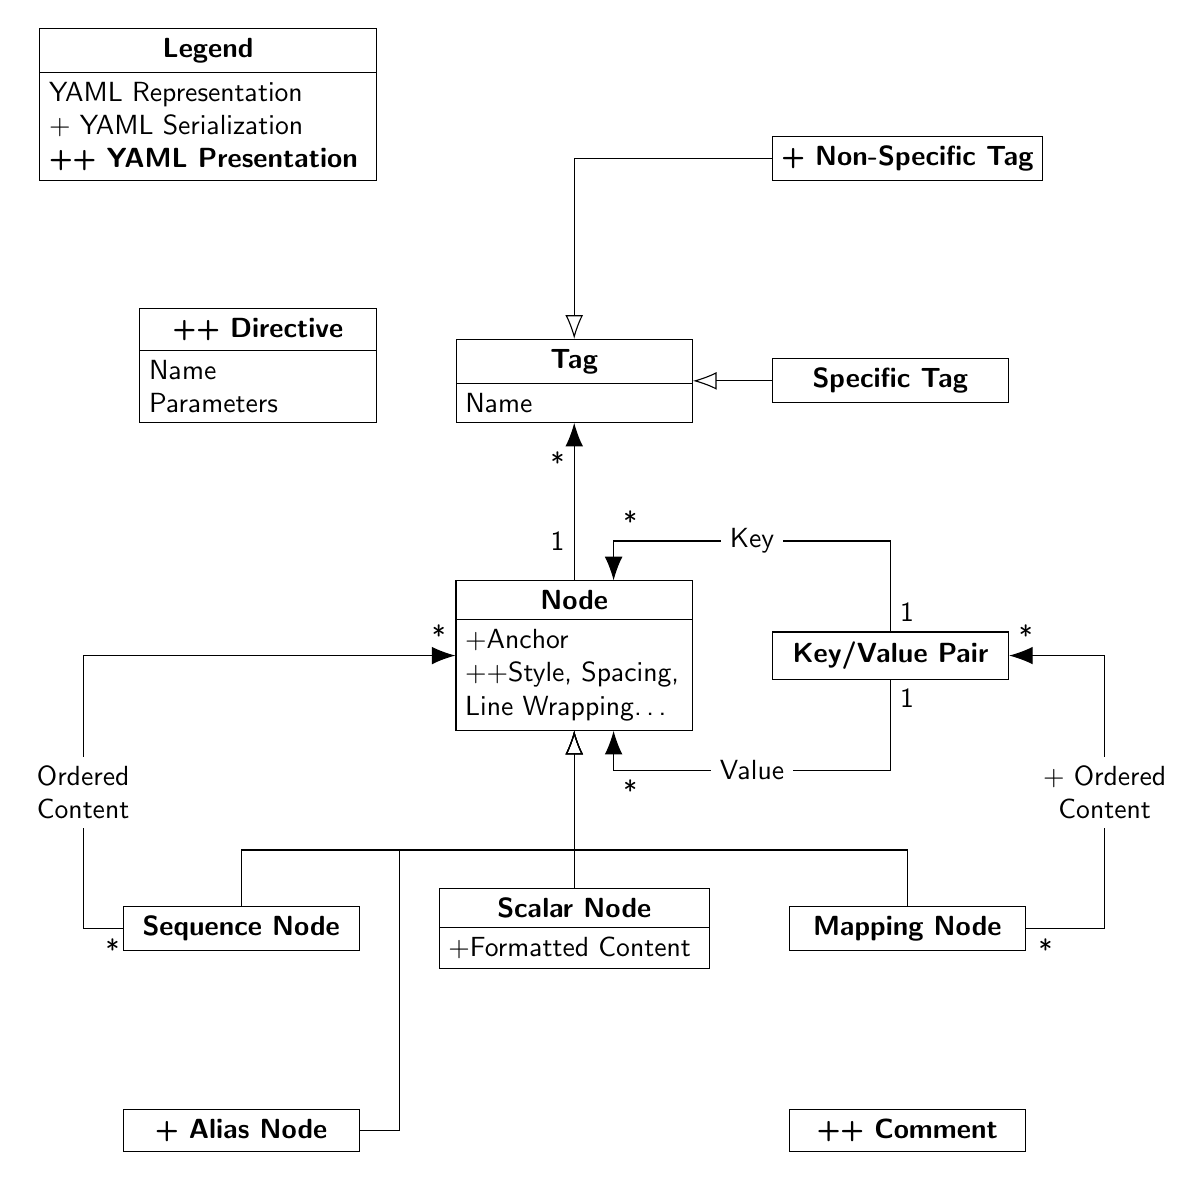
\begin{tikzpicture}

\entity{Node}{
  +Anchor\\
  ++Style, Spacing,\\
  Line Wrapping…
};

\entity[above=of Node]{Tag}{Name};
\draw[has] (Node) -- (Tag)
  node[near start, left]{1}
  node[near end, left]{*};

\entity[right=of Tag]{Specific Tag}{};
\draw[inherits] (Specific Tag) -- (Tag);

\entity[above right=of Tag]{+ Non-Specific Tag}{};
\draw[inherits] (+ Non-Specific Tag) -| (Tag);

\entity[below=of Node]{Scalar Node}{+Formatted Content};
\draw[inherits] (Scalar Node) -- (Node);

\entity[left=of Scalar Node]{Sequence Node}{};
\draw[inherits] (Sequence Node) -- ++(0,+10mm) -| (Node);

\draw[has] (Sequence Node.west)
  -- ++(-5mm, 0) node[near start, below] {*}
  |- (Node) node[onArrow, pos=0.25] {Ordered\\Content}
  node[at end, above left] {*};

\entity[below=of Sequence Node]{+ Alias Node}{};
\draw[inherits]
  let
    \p1 = ($(+ Alias Node.east)+(5mm,0)$),
    \p2 = ($(Sequence Node)+(0,10mm)$)
  in
  (+ Alias Node) -| (\x1,\y2) -| (Node)
;

\entity[right=of Scalar Node]{Mapping Node}{};
\draw[inherits] (Mapping Node) -- ++(0,+10mm) -| (Node);

\entity[right=of Node]{Key/Value Pair}{};

\draw[has]
  (Mapping Node.east)
  -- ++(10mm, 0) node[near start, below] {*}
  |- (Key/Value Pair) node[onArrow, pos=0.25] {+ Ordered\\Content}
  node[at end, above right] {*};

\draw[has] (Key/Value Pair.north)
  |- ($(Node.north)+(0.5,0.5)$)
  node[at start, above right] {1}
  node[pos=0.75, onArrow] {Key}
  -- ($(Node.north)+(0.5,0)$)
  node[at start, above right] {*};

\draw[has] (Key/Value Pair.south)
  |- ($(Node.south)+(0.5,-0.5)$)
  node[at start, below right] {1}
  node[pos=0.75, onArrow] {Value}
  -- ($(Node.south)+(0.5,0)$)
  node[at start, below right] {*};

\entity[below=of Mapping Node]{++ Comment}{}

\entity[above left=of Node]{++ Directive}{Name\\Parameters}

\entity[above left=of Tag]{Legend}{
  YAML Representation\\
  + YAML Serialization\\
  \textbf {++ YAML Presentation}
}

\end{tikzpicture}

\end{document}
